\subsubsection{Presentation Layer}
\begin{figure}[H]
    \centering
    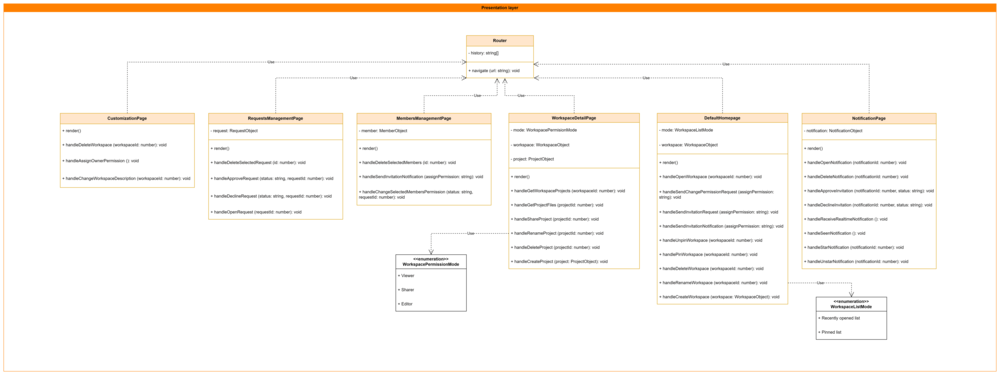
\includegraphics[ width = \linewidth]{Content/Phân tích và thiết kế hệ thống/documents/Sơ đồ lớp/images/Presentation layer/presentationLayer.png}
    \vspace{0.5cm}
    \caption{Tổng quan Presentation Layer}
    \label{fig:Tổng quan Presentation layer}
\end{figure}
Tầng presentation biểu diễn những giao diện được hiện thực, nó sẽ bao gồm cả những trạng thái (mode) của giao diện cũng như những hàm hiện thực chức năng logic của giao diện tương ứng.
Chi tiết cụ thể hơn sẽ được trình bày trong phần dưới theo từng class được hiện thực.

\begin{figure}[H]
    \centering
    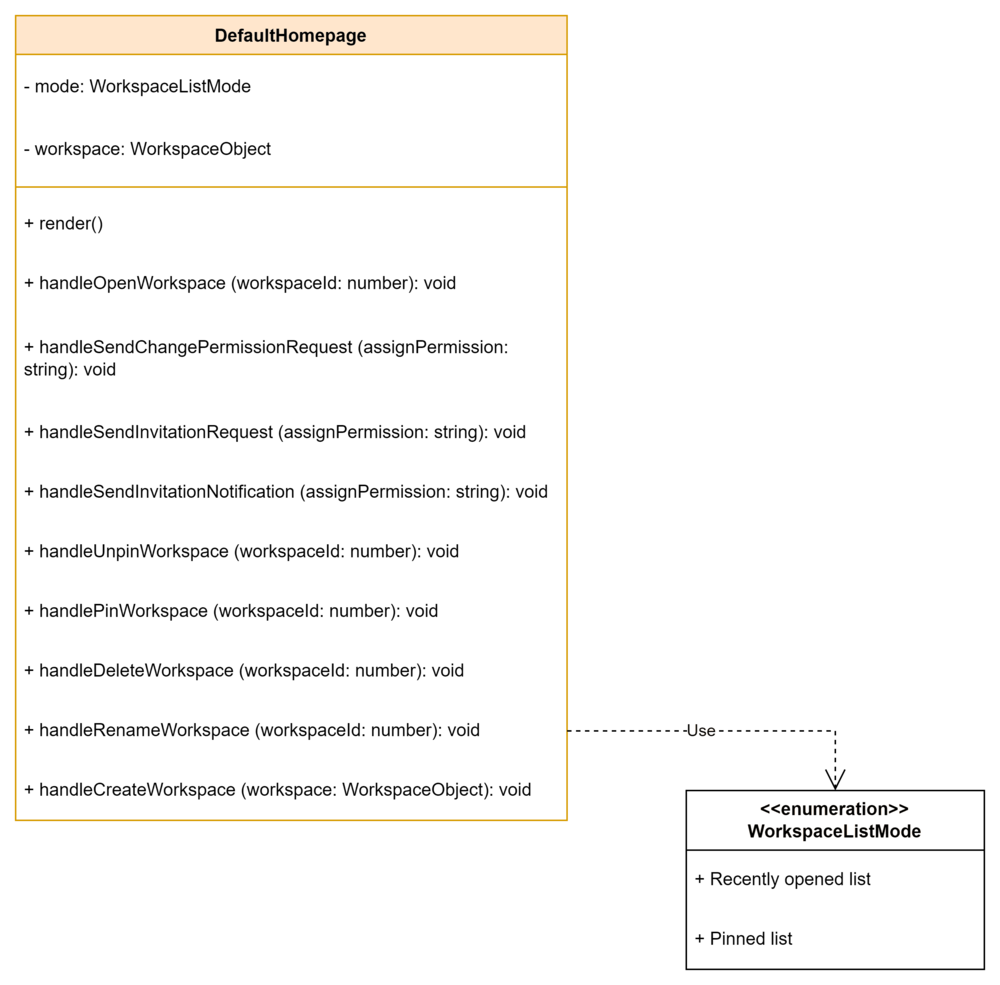
\includegraphics[ width = 0.7\linewidth]{Content/Phân tích và thiết kế hệ thống/documents/Sơ đồ lớp/images/Presentation layer/defaultWorkspacePage.png}
    \vspace{0.5cm}
    \caption{Class DefaultHomepage trong Presentation layer}
    \label{fig:Class Default homepage trong Presentation layer}
\end{figure}
Ở giao diện mặc định khi người dùng được chuyển hướng tới sau khi hoàn tất thủ tục xác thực với hệ thống, chúng ta sẽ tập trung vào những chức năng liên quan tới việc hiển thị và tương tác với workspace mà người dùng tham gia (create, open, pin, delete, rename). Những chức năng đáng chú ý là nhóm chức năng gửi lời mời vào workspace/gửi yêu cầu mời người dùng khác vào workspace, nhóm chức năng này được xử lý real-time (thời gian thực) để nhận và hiển thị dữ liệu ở những giao diện khác. Giao diện sẽ có hai hình thức hiển thị danh sách workspace là theo thời gian mở workspace gần nhất - "Recently opened workspace" và những workspace được người dùng ghim thủ công - "Pinned workspace".

\begin{figure}[H]
    \centering
    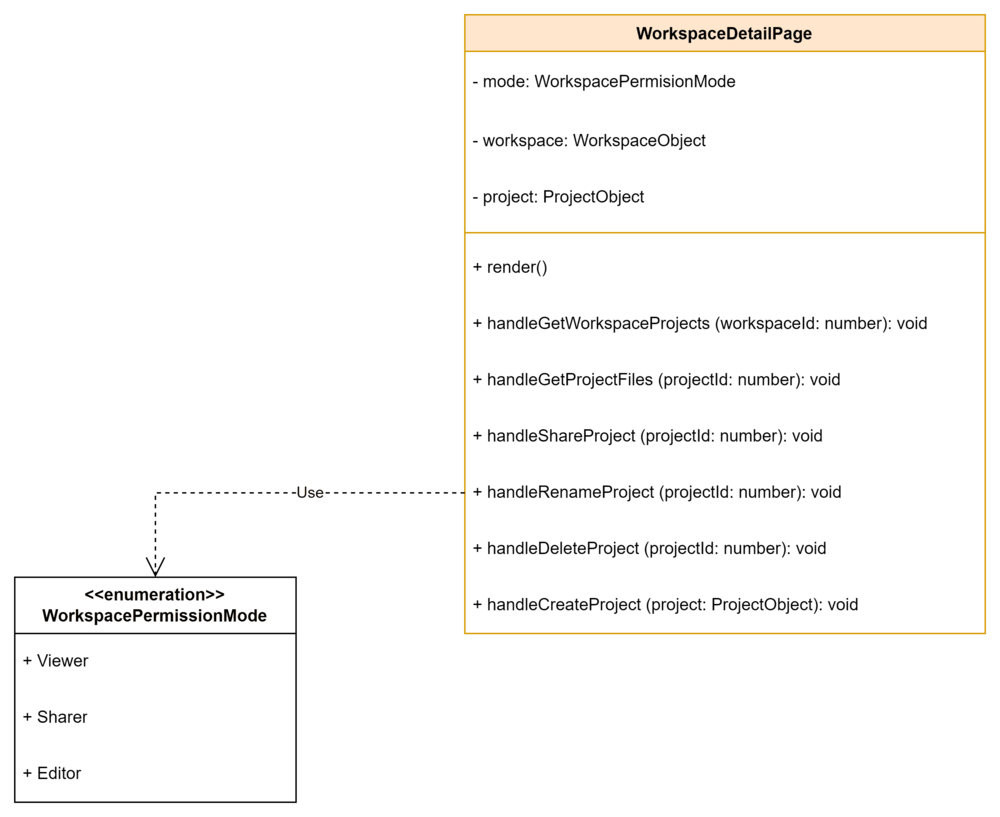
\includegraphics[ width = 0.7\linewidth]{Content/Phân tích và thiết kế hệ thống/documents/Sơ đồ lớp/images/Presentation layer/workspaceDetailPage.png}
    \vspace{0.5cm}
    \caption{Class WorkspaceDetailPage trong Presentation layer}
    \label{fig:Class WorkspaceDetailPage trong Presentation layer}
\end{figure}
Người dùng sẽ được chuyển hướng tới giao diện hiển thị nội dung bên trong workspace khi sử dụng chức năng "Open workspace" hoặc chọn item workspace tương ứng, nội dung bên trong workspace sẽ được hiển thị dưới dạng danh sách những project có bên trong workspace. Mỗi project sẽ là bao gồm nhiều process/version của process và document bên trong. Người dùng sẽ được phân quyền hạn khi tham gia vào workspace: viewer, sharer và editor.

\begin{figure}[H]
    \centering
    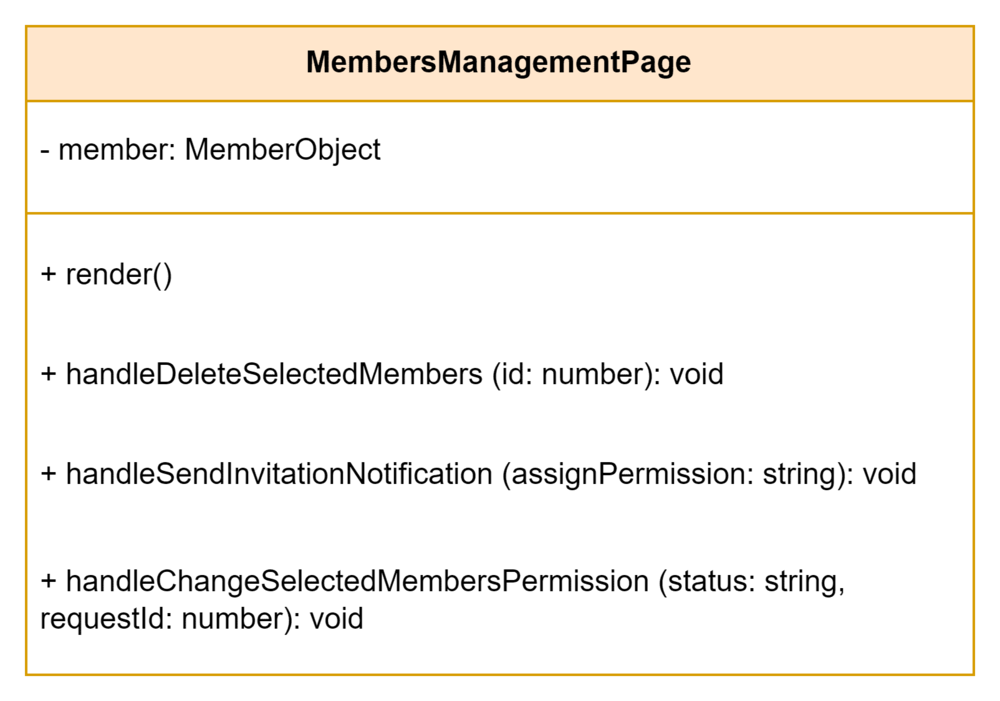
\includegraphics[ width = 0.5\linewidth]{Content/Phân tích và thiết kế hệ thống/documents/Sơ đồ lớp/images/Presentation layer/membersManagementPage.png}
    \vspace{0.5cm}
    \caption{Class MemberManagementPage trong Presentation layer}
    \label{fig:Class MemberManagementPage trong Presentation layer}
\end{figure}
Giao diện quản lý thành viên trong workspace là mục mặc định được điều hướng khi người sở hữu workspace chuyển hướng tới giao diện quản lý. Class này sẽ tập trung hiện thực những chức năng liên quan tới thêm/xóa thành viên trong workspace và điều chỉnh quyền hạn của thành viên tương ứng trong workspace. Ngoài ra còn có chức năng gửi lời mời vào workspace cho người dùng khác, chức năng này cũng sẽ được xử lý real-time để hiển thị dữ liệu ở giao diện thông báo cá nhân khi người dùng khác nhận được lời mời.

\begin{figure}[H]
    \centering
    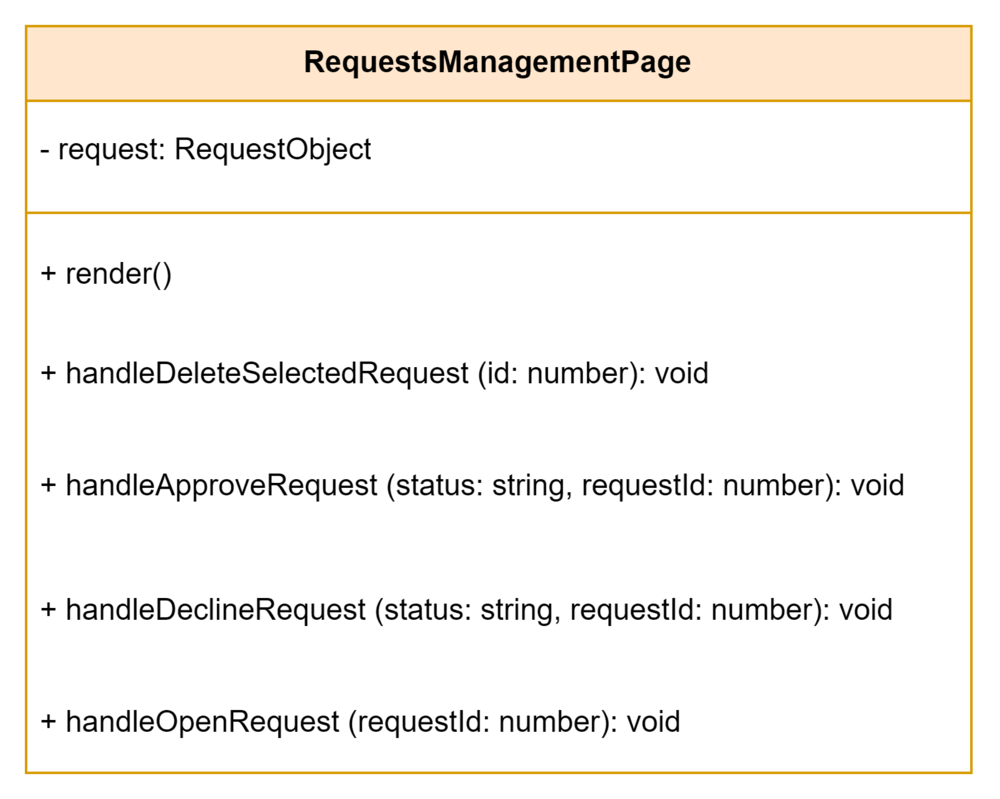
\includegraphics[ width = 0.5\linewidth]{Content/Phân tích và thiết kế hệ thống/documents/Sơ đồ lớp/images/Presentation layer/requestManagementPage.png}
    \vspace{0.5cm}
    \caption{Class RequestManagementPage trong Presentation layer}
    \label{fig:Class RequestManagementPage trong Presentation layer}
\end{figure}
Giao diện quản lý yêu cầu sẽ hiển thị những yêu cầu nhận được từ thành viên bên trong workspace. Những yêu cầu này sẽ được hiển thị dưới dạng danh sách và được phân loại theo loại yêu cầu và trạng thái xử lý của chúng (pending - chờ xử lý, approved - đồng ý hay declined - từ chối).

\begin{figure}[H]
    \centering
    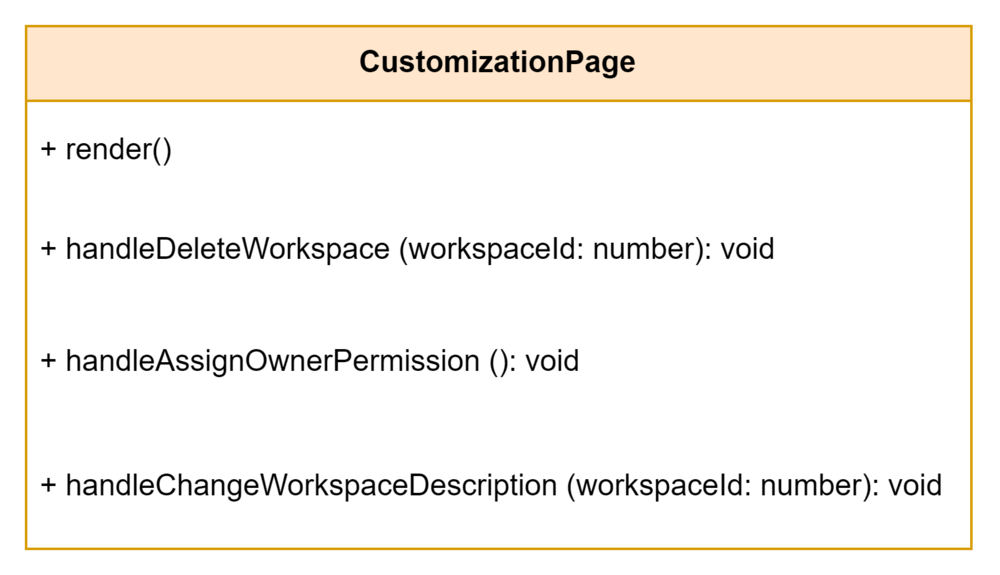
\includegraphics[ width = 0.5\linewidth]{Content/Phân tích và thiết kế hệ thống/documents/Sơ đồ lớp/images/Presentation layer/customizationPage.png}
    \vspace{0.5cm}
    \caption{Class CustomizationPage trong Presentation layer}
    \label{fig:Class CustomizationPage trong Presentation layer}
\end{figure}
Giao diện này sẽ hiện thực những chức năng dành cho người sở hữu workspace như xóa workspace, chuyển quyền sở hữu workspace cho thành viên khác hoặc thay đổi mô tả chi tiết của workspace.

\begin{figure}[H]
    \centering
    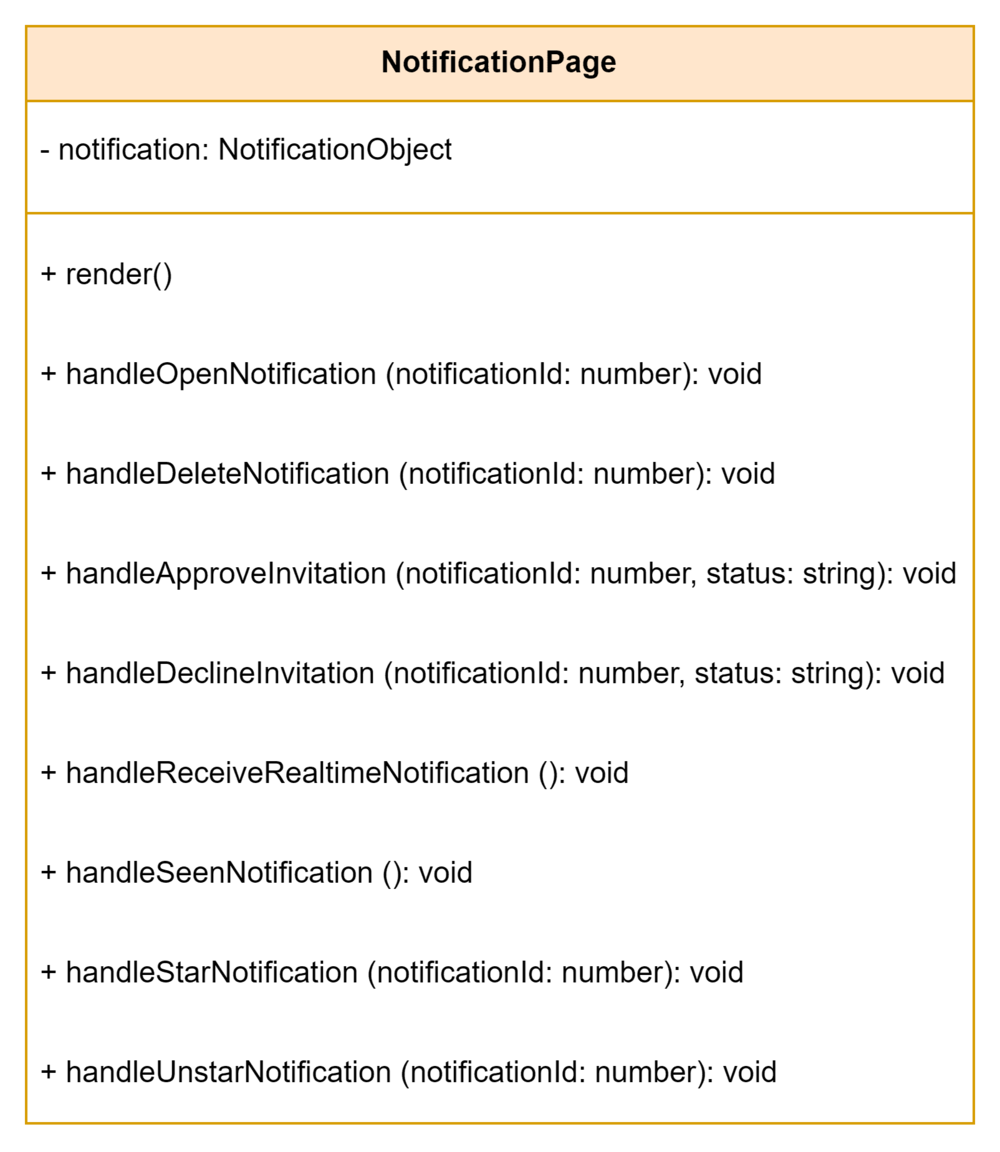
\includegraphics[ width = 0.5\linewidth]{Content/Phân tích và thiết kế hệ thống/documents/Sơ đồ lớp/images/Presentation layer/notificationPage.png}
    \vspace{0.5cm}
    \caption{Class NotificationPage trong Presentation layer}
    \label{fig:Class NotificationPage trong Presentation layer}
\end{figure}
Giao diện thông báo cá nhân là giao diện phụ trách việc hiển thị và giúp người dùng phản hồi những thông báo gửi đến họ. Sẽ có nhiều loại thông báo nhưng trong đó sẽ có thông báo yêu cầu xác nhận từ người dùng (lời mời vào workspace của thành viên trong workspace), hệ thống còn ghi nhận những thông báo đã được đọc và trạng thái của chúng để giúp người dùng có trải nghiệm tốt hơn khi truy xuất những thông báo cần xử lý.